\section{Aim}
 To study aggregate function: SUM, COUNT, AVG, MAX, MIN.

\section{{Theory}}

The Aggregate Functions in SQL are: 
\begin{itemize}
	\item SUM(): Used to find the sum of the values over a column
	\item MIN(): Used to find the minimum value in a column.
	\item MAX(): Used to find the maximum value in a column.
	\item AVG(): Used to find the average over a column.
	\item COUNT(): Used to count the number of rows in the output.
\end{itemize}

\section{{Code and Output}}

\begin{enumerate}
\item Find the class average for the subject ‘Physics’\newline
\begin{minted}{sql}

SELECT AVG(physics) FROM students;

\end{minted}
\newline
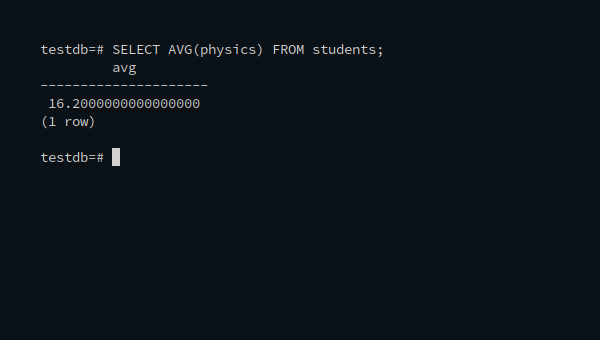
\includegraphics[width=\linewidth]{../Images/Aggregate/1.png}\newline
\item Find the highest marks for mathematics (To be displayed as highest\_marks\_maths).\newline
\begin{minted}{sql}

SELECT MAX(maths) AS highest_marks_maths FROM students;

\end{minted}
\newline
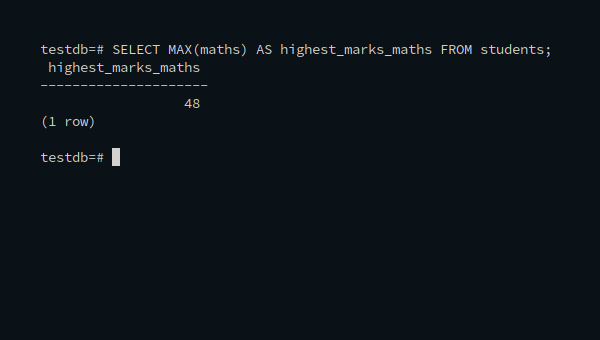
\includegraphics[width=\linewidth]{../Images/Aggregate/2.png}\newline
\item Find the lowest marks for chemistry(To be displayed as lowest\_mark\_chemistry)\newline
\begin{minted}{sql}

SELECT MIN(chemistry) AS lowest_marks_chemistry 
	FROM students;

\end{minted}
\newline
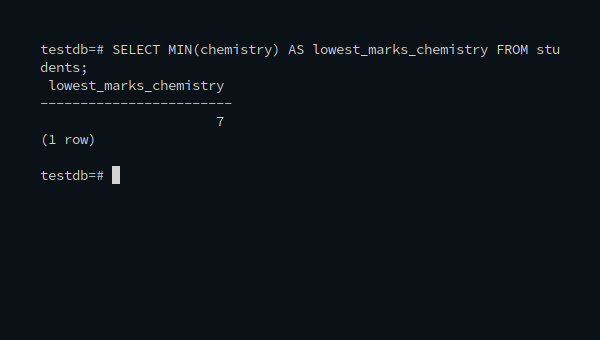
\includegraphics[width=\linewidth]{../Images/Aggregate/3.png}\newline
\item Find the total number of students who has got a ‘pass’ in physics.\newline
\begin{minted}{sql}

SELECT COUNT(*) AS passed_physics FROM students 
	WHERE physics > 12;

\end{minted}
\newline
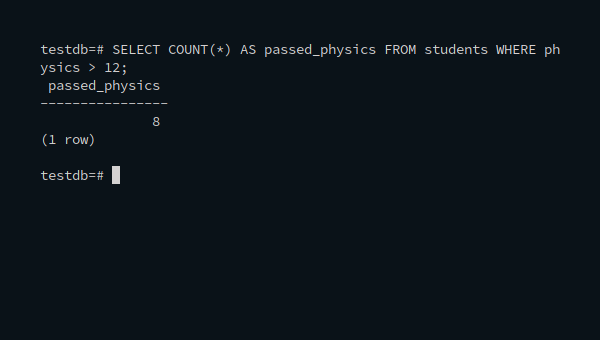
\includegraphics[width=\linewidth]{../Images/Aggregate/4.png}\newline
\item Generate the list of students who have passed in all the subjects\newline
\begin{minted}{sql}

SELECT * FROM students 
	WHERE physics > 12 AND chemistry > 12 AND maths > 25;

\end{minted}
\newline
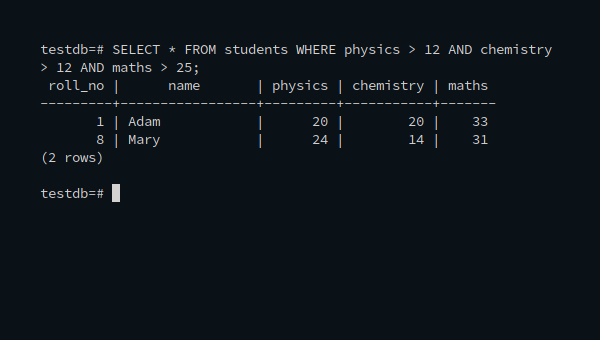
\includegraphics[width=\linewidth]{../Images/Aggregate/5.png}\newline
\item Generate a rank list for the class.Indicate Pass/Fail. Ranking based on total marks obtained by the
students.\newline
\begin{minted}{sql}

ALTER TABLE students ADD COLUMN result CHAR(1);
UPDATE students SET result = 'P' 
	WHERE physics > 12 AND chemistry > 12 AND maths > 25
UPDATE students SET result = 'F' 
	WHERE physics < 12 OR chemistry < 12 OR maths < 25
UPDATE students 
	SET total_marks = chemistry+physics+maths;
SELECT * FROM students ORDER BY total_marks;

\end{minted}
\newline
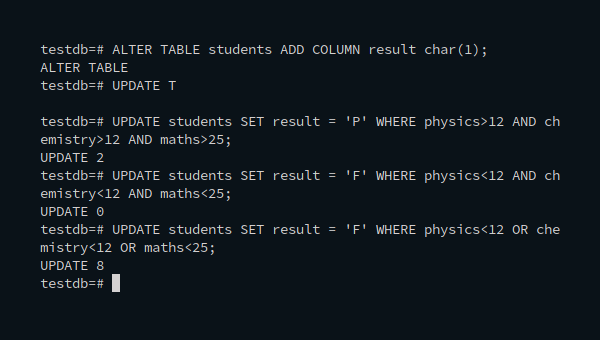
\includegraphics[width=\linewidth]{../Images/Aggregate/6.png}
\newline
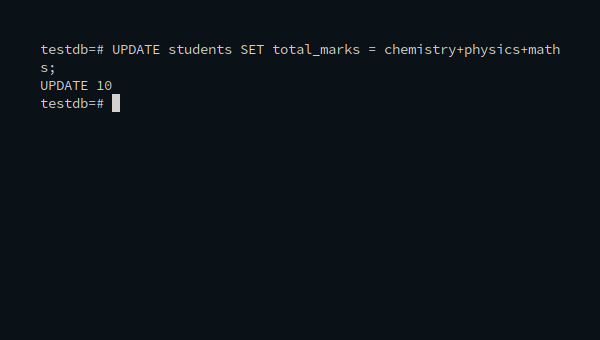
\includegraphics[width=\linewidth]{../Images/Aggregate/7.png}
\newline
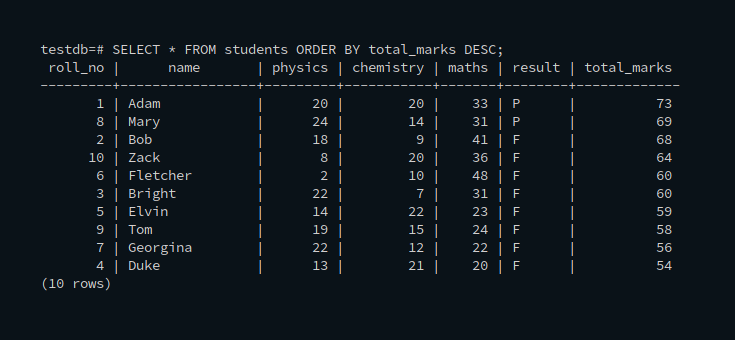
\includegraphics[width=\linewidth]{../Images/Aggregate/8.png}\newline
\item Find pass percentage of the class for mathematics.\newline
\begin{minted}{sql}

SELECT COUNT(*) * 100 / (SELECT COUNT(*) FROM students) 
	AS pass_perc_maths FROM students WHERE maths > 25;

\end{minted}
\newline
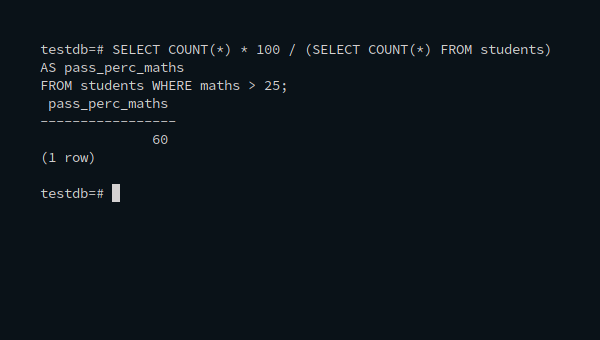
\includegraphics[width=\linewidth]{../Images/Aggregate/10.png}\newline
\item Find the overall pass percentage for all class.\newline
\begin{minted}{sql}

SELECT COUNT(*) * 100 / (SELECT COUNT(*) FROM students) 
	AS pass_perc FROM students 
	WHERE maths > 25 AND physics > 12 and chemistry > 12;

\end{minted}
\newline
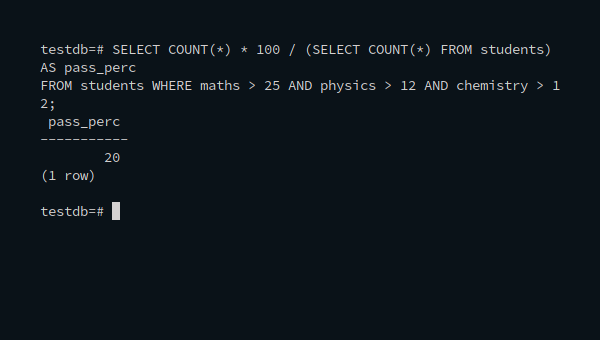
\includegraphics[width=\linewidth]{../Images/Aggregate/11.png}\newline
\item Find the class average.\newline
\begin{minted}{sql}

SELECT AVG(total_marks) FROM students;

\end{minted}
\newline
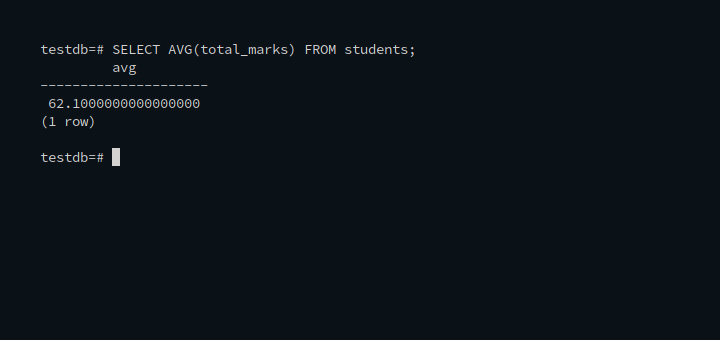
\includegraphics[width=\linewidth]{../Images/Aggregate/12.png}\newline
\item Find the total number of students who have got a Pass.\newline
\begin{minted}{sql}

SELECT COUNT(*) FROM students WHERE result = 'P';

\end{minted}
\newline
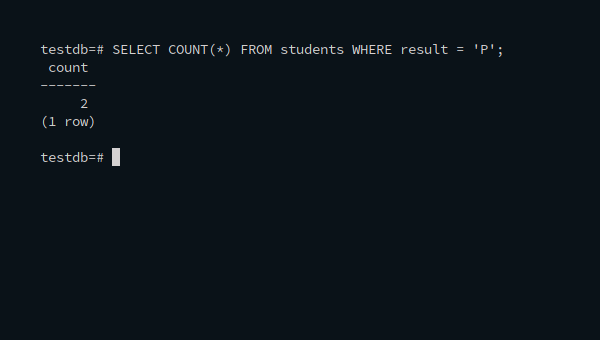
\includegraphics[width=\linewidth]{../Images/Aggregate/13.png}\newline
\end{enumerate}

\section{Result}
Implemented the program for Aggregate Functions using Postgresql 11.5 on Manjaro Linux and the output was obtained.